\twocolumn[{\begin{figure}[H]
	\setlength{\linewidth}{\textwidth}
	\setlength{\hsize}{\textwidth}
	\centering
	\centering
	\begin{tikzpicture}
		\node[anchor=north west] at (0,0){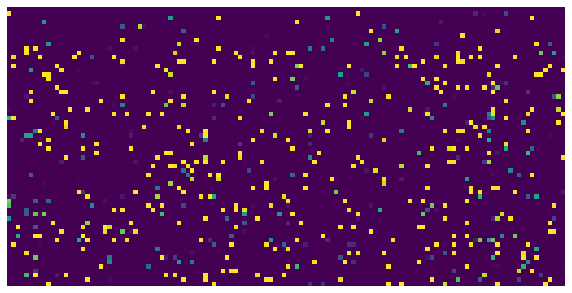
\includegraphics[width=4cm]{errors_18_2}};
		\node[anchor=north west] at (4,0){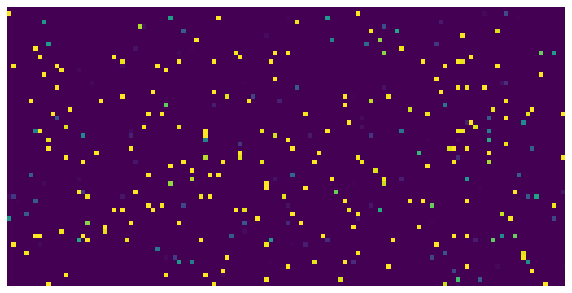
\includegraphics[width=4cm]{errors_18_2_1to0}};
		\node[anchor=north west] at (8,0){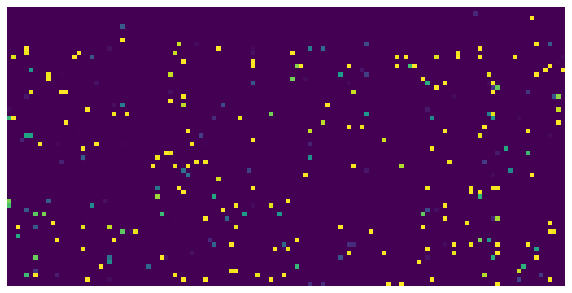
\includegraphics[width=4cm]{errors_18_2_0to1}};
		\node[anchor=north west] at (12,0){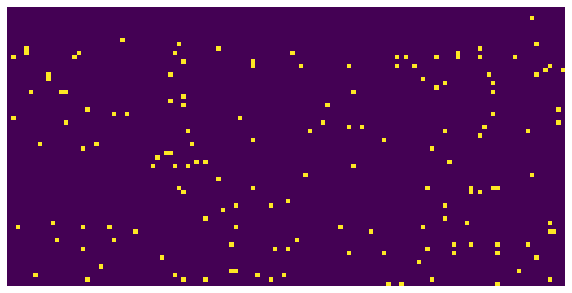
\includegraphics[width=4cm]{errors_18_2_sa1}};
		
		\node[anchor=north west] at (0,-2.5){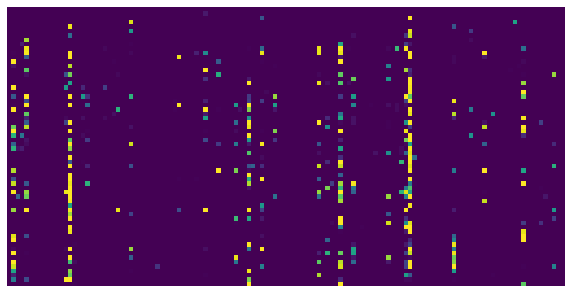
\includegraphics[width=4cm]{errors_n_2}};
		\node[anchor=north west] at (4,-2.5){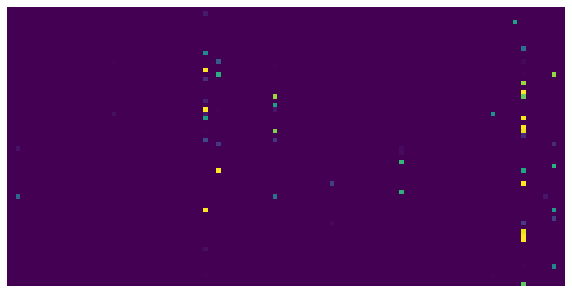
\includegraphics[width=4cm]{errors_n_2_1to0}};
		\node[anchor=north west] at (8,-2.5){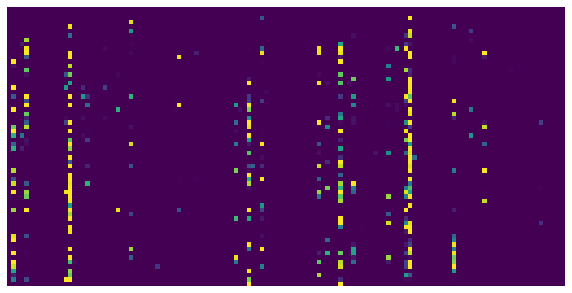
\includegraphics[width=4cm]{errors_n_2_0to1}};
		\node[anchor=north west] at (12,-2.5){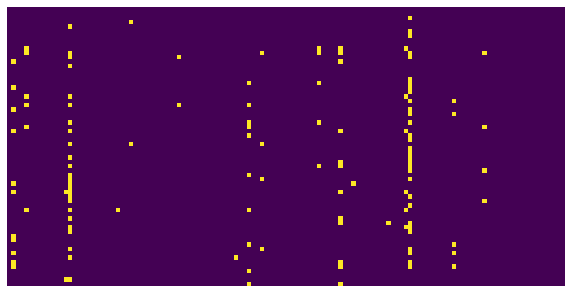
\includegraphics[width=4cm]{errors_n_2_sa1}};
		
		\node[anchor=south east,fill opacity=0.75,fill=white] at (4, -2){$p{\approx}2.75\%$};
		\node[anchor=south east,fill opacity=0.75,fill=white] at (4, -4.5){$p{\approx}1.08\%$};
		
		\draw[white!30!black,-, line width=0.75pt] (12.125,-5.1) -- (12.125,0.4);
		\draw[thick,->] (0.05,0.05) -- (1,0.05);
		\draw[thick,->] (-0.05,-0.05) -- (-0.05,-1);
		\node[anchor=south] at (0.75,0.05){128 columns};
		\node[rotate=90,anchor=south] at (-0.05,-0.6){64 rows};
		
		\node[anchor=south] at (6,-0.2) {\bfseries Chip 1};
		\node[anchor=north] at (6,-2.2) {\bfseries Chip 2};
		
		\node at (2, -5){Overall bit flips};
		\node at (4, -5){=};
		\node at (6, -5){$1$-to-$0$ flips};
		\node at (8, -5){+};
		\node at (10, -5){$0$-to-$1$ flips};
		\node at (14, -5){persistent errors};
	\end{tikzpicture}
	\vspace*{-6px}
	\caption{\textbf{Low-Voltage Induced Bit Errors on Profiled Chips.} Complementary to \figref{fig:errors}, we break the the bit error distribution of chips 1 and 2 down into $1$-to-$0$ and $0$-to-$1$ bit flips. Additionally, most of the bit errors are actually persistent across accesses at a given supply voltage. As before, we show a sub-array of size $64 \times 128$ from all profiled bit cells (\ie, across all SRAM arrays). \secref{sec:supp-introduction} includes details on profiling.}
	\label{fig:supp-errors}
	\vspace*{-0.1cm}
\end{figure}}]

\section{Energy Savings in \figref{fig:introduction}}
\label{sec:supp-introduction}

\figref{fig:introduction} shows bit error rate characterization results of SRAMs in the DNN accelerator chip described in \cite{ChandramoorthyHPCA2019}, fabricated using 14nm FinFET technology. The average bit error rate is measured from 32 SRAMs, each SRAM array of size 4KB (512 $\times$ 64 bit), as supply voltage is scaled down. \textit{Bit error rate} $p$ (in \%) at a given supply voltage is measured as the count of read or write bit cell failures averaged over the total number of bit cells in the SRAM. A bit cell failure refers to reading 1 on writing 0 or reading 0 on writing 1.  For a more comprehensive characterization of SRAMs in 14nm technology, the reader is referred to \cite{GanapathyDAC2017}. \figref{fig:introduction} also shows the energy per write and read access of a 4KB (512 $\times$ 64 bit) SRAM, obtained from Cadence Spectre simulations. Energy is obtained at the same constant clock frequency at all supply voltages. The voltage (x-axis) shown is normalized over \Vmin which is the lowest measured voltage at which there are no bit cell failures.  Energy shown in the graph (secondary axis on the right) is also normalized over the energy per access at \Vmin.

Accelerators such as \cite{ChenISCA2016,ChenASPLOS2014,ChandramoorthyHPCA2019, ReagenISCA2016, nvdla, DuISCA2015,SharmaISCA2018} have a large amount of on-chip SRAM to store weights and intermediate computations. Total dynamic energy of accelerator SRAMs can be obtained as the total number of SRAM accesses times the energy of a single SRAM access. Optimized dataflow in accelerators leads to better re-use of weights read from memories in computation, reducing the number of such memory accesses ~\cite{ChenISCA2016,ChenASPLOS2014, nvdla}. Low voltage operation focuses on reducing the memory access energy, leading to significant energy savings as shown. 